% !TEX TS-program = xelatex
% !TEX encoding = UTF-8 Unicode
% !Mode:: "TeX:UTF-8"

\documentclass{resume}
\usepackage{graphicx}
\usepackage{tabu}
\usepackage{tabularx}
\usepackage{multirow}
\usepackage{progressbar}
\usepackage{zh_CN-Adobefonts_external} % Simplified Chinese Support using external fonts (./fonts/zh_CN-Adobe/)
\usepackage{tikz}
% \usepackage{NotoSansSC_external}
% \usepackage{NotoSerifCJKsc_external}
% \usepackage{zh_CN-Adobefonts_internal} % Simplified Chinese Support using system fonts
\usepackage{linespacing_fix} % disable extra space before next section
\usepackage{cite}

\newcommand{\hlink}[1]{\href{#1}{#1}}

\begin{document}
\pagenumbering{gobble} % suppress displaying page number

\medskip\noindent
\begin{minipage}{0.7\textwidth}
  \Large{
    \begin{tabu}  { l }
      \scshape{徐 \quad  颖} \\
      \email{xuying1706@buaa.edu.cn} \\
      \phone{(+86) 131-2661-1215} \\
    \end{tabu}
  }
\end{minipage}
\begin{minipage}{0.3\textwidth}
  \raggedleft
  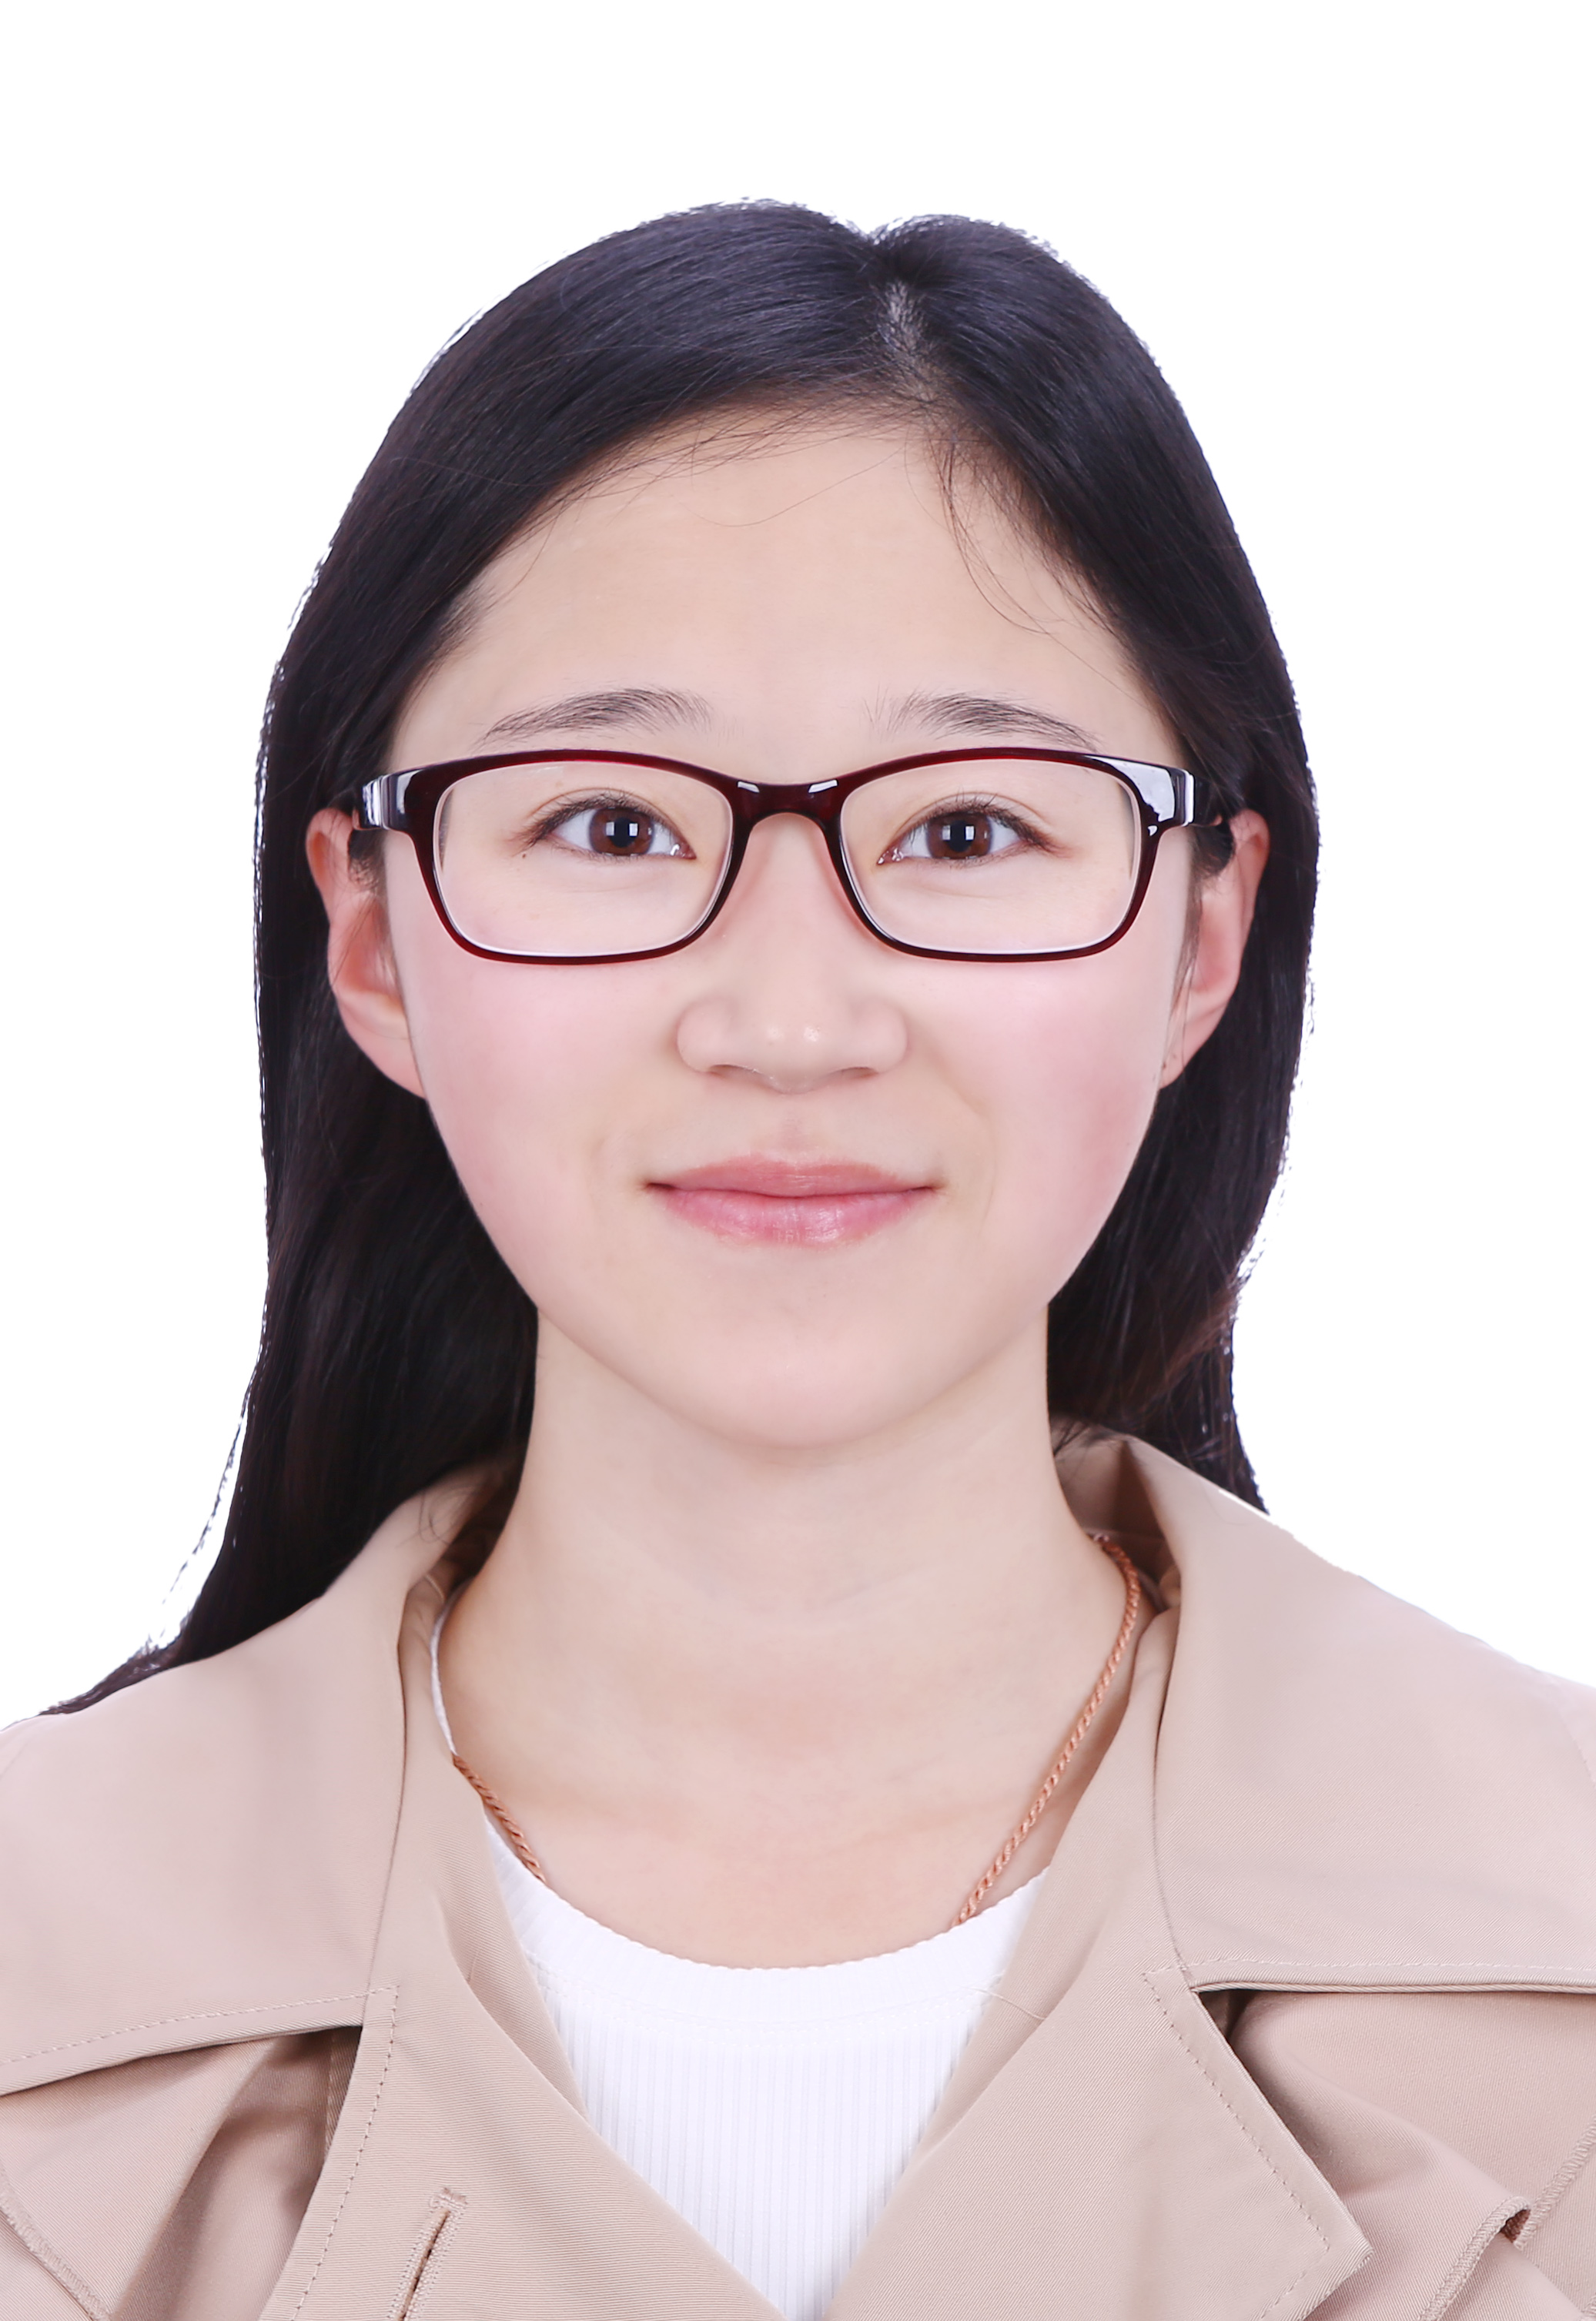
\includegraphics[height=30mm]{xy}
\end{minipage}



\section{  教育背景}
\datedsubsection{\textbf{北京航空航天大学}, 北京}{2017.08 -- 至今}
\textit{在读硕士研究生}\quad {计算机学院}
\datedsubsection{\textbf{南开大学}, 天津}{2013.09 -- 2017.07}
\textit{学士}\quad  {计算机与控制工程学院}

\section{ 实习/项目经历}

\datedsubsection{\textbf{对抗攻击}}{2018.10 -- 至今}
\role{研究生课题}{}
%\begin{onehalfspacing}
\begin{itemize}[topsep = 0 pt, partopsep = 0pt]
  \item 使用DAG算法对FCN和Faster-RCNN进行攻击
  \item 使用GAN对Two-Stream动作识别模型进行攻击
\end{itemize}
%\end{onehalfspacing}


\datedsubsection{\textbf{目标检测}}{2018.02 -- 2018.09}
\role{研究生课题}{}
%\begin{onehalfspacing}
\begin{itemize}[topsep = 0 pt, partopsep = 0pt]
  \item 使用Faster-RCNN和Mask RCNN进行目标检测
\end{itemize}
%\end{onehalfspacing}

\datedsubsection{\textbf{基于时空分解的民航旅客流量分析与预测}}{2016.06 -- 2017.06}
\role{本科毕设}{}
\begin{itemize}[topsep = 0 pt, partopsep = 0pt]
  \item 对民航客流量大数据进行清洗和统计
  \item 深入分析民航旅客在时间和空间上的出行规律
  \item 建立民航领域的时空残差网络模型,对航线的日客流量进行预测
\end{itemize}

% \datedsubsection{\textbf{基于虚拟现实技术的医学影像重建与交互系统}}{2016.6 -- 2017.6}
% \role{Unity3D}{本科毕设,北航电子实验中心}
% %\begin{onehalfspacing}
% \begin{itemize}[topsep = 0 pt, partopsep = 0pt]
%   \item CT、MRI等医疗影像的三维重建
%   \item HTC Vive虚拟显示设备的显示与交互
%   \item 可使用VR设备对三维人体模型切片,观察内部结构,辅助诊断与教学
% \end{itemize}
% %\end{onehalfspacing}


\section{学生工作}
    \datedline{\textit{CCF北航学生分会主席}}{2018.12 -- \  \quad 至今}
    \datedline{\textit{CCF北航学生分会副主席}}{2017.11 -- 2018.12}
    \datedline{\textit{南开大学360俱乐部组织部组长}}{2015.03 -- 2017.06}
    \datedline{\textit{南开大学豌豆藤志愿服务组织小组组长}}{2013.10 -- 2017.06}

\section{技能}
% increase linespacing [parsep=0.5ex]
\begin{itemize}[parsep=0.5ex]
  \item 语言: CET-6 547
  \item 编程语言:常用C++、MATLAB、Python,了解SQL
  \item 框架: PyTorch、Caffe
  \item 工具: Linux、Git、MySQL、SQL Server
\end{itemize}

\section{获奖情况}
\datedline{\textit{北京航空航天大学新生奖学金}}{2017.08}
\datedline{\textit{北京航空航天大学学业奖学金}}{2018.08}

% \section{ 其他}
% % increase linespacing [parsep=0.5ex]
% \begin{itemize}[parsep=0.5ex]
%   \item  英语 - 熟练(CET-6 530)
%   \item  无线电台呼号 BI1GPX
% \end{itemize}

\end{document}
